\section{Application Demonstration}
\label{sec:demo}
 
\begin{figure*}[]
	\centering
	{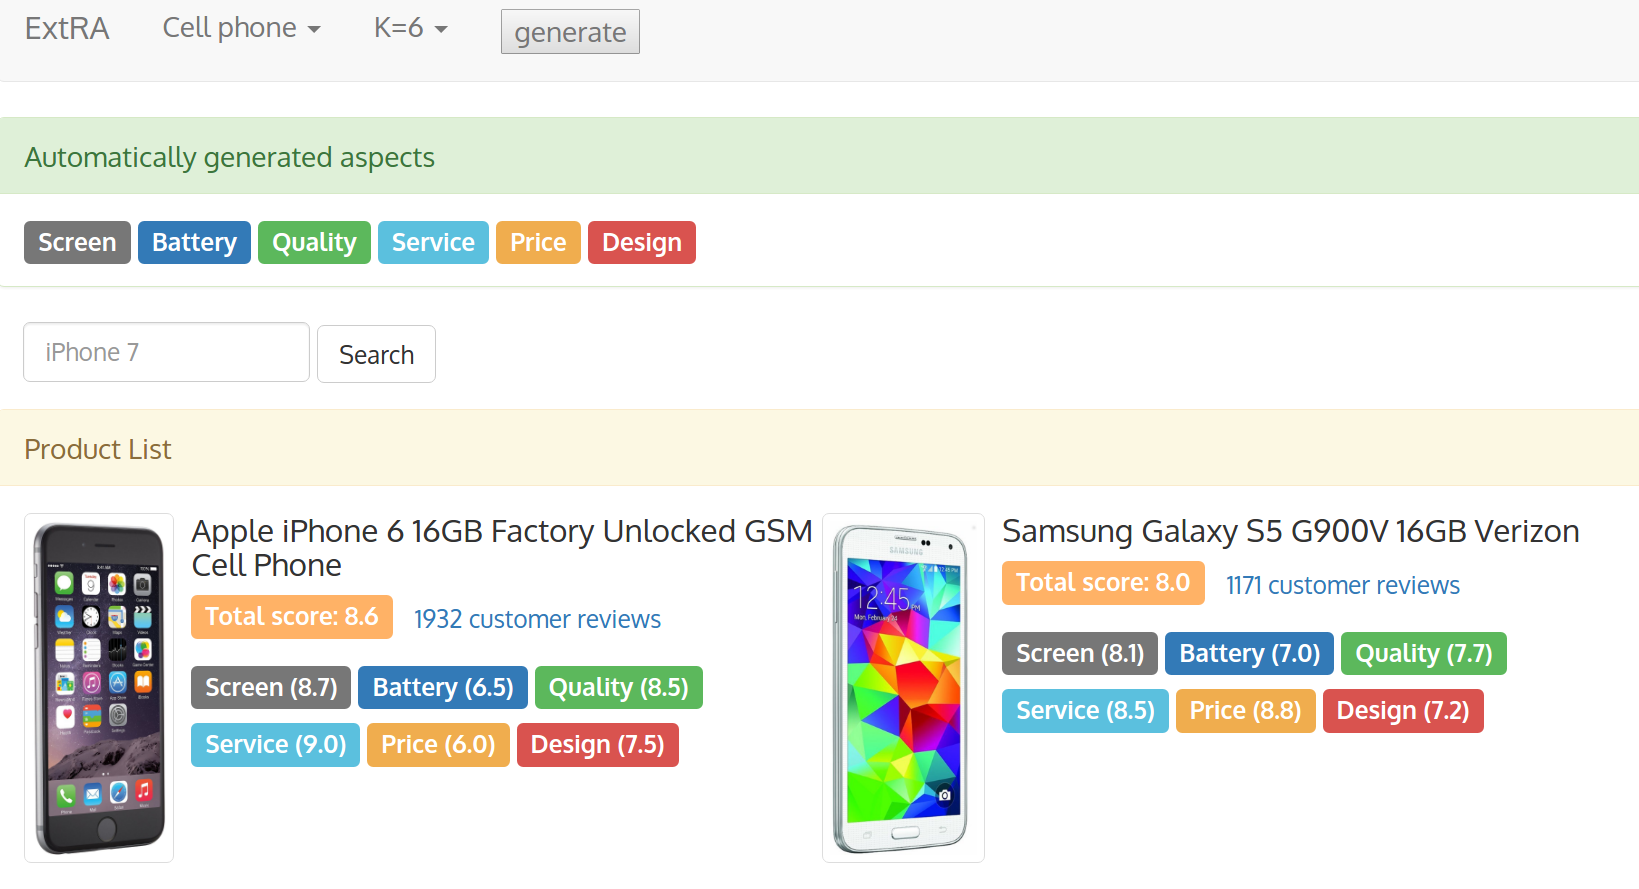
\includegraphics[width=1.5\columnwidth]{figures/sentimentcompare.png}}\vfill 
	\caption{Automatically generated 6 aspects for mobile phones\label{fig:experiments:sentimentcompare}}
\end{figure*}
A most important downstream application of our extracted prominent review aspects is \textit{aspect-based sentiment analysis on user reviews}.
In this section,
we demonstrate a real instance of such application, developed with the results from our framework ExtRA.
%\footnote{Our demo system is available at \url{http://anonymized.due.to.blind.review}} 
%based on our proposed aspect extraction framework ExtRA. 

With the application, people can specify their expected number of prominent aspects $K$ for a certain product type.
Then, they can investigate the sentiment of existing customers towards any products under this type from the most prominent aspects extracted by ExtRA.
%User can select a product type from a predefined set of categories, 
%and specify the number of expect aspects $K$. 

\figref{fig:experiments:sentimentcompare} shows a snapshot
of our application when users are investigating the cell phone reviews based on $K=6$ extracted prominent aspects. 
The topic clusters extracted from mobile phones review texts are shown
in \tabref{table:clusters}.
%The topic clusters by our method on the mobile phones review data is shown in \tabref{table:clusters}.  
%We use the top aspect words extracted by our model to represent clusters (in this example, we set $K=6$). 
%The user may filter out some of the results by using the search box. 
We propose a scoring method for review summarization in our demo system. 
As the running example shown in \figref{fig:experiments:sentimentcompare},
each kind of mobile phone has rating scores summarized on each extracted prominent review aspect.
The scores are computed by sentiment analysis of reviews containing the prominent aspects.
We calculate the sentiment score of each aspect by analyze the sentiment of all sentences containing this aspect term.
Using \textit{Deeply Moving}\footnote{\url{https://nlp.stanford.edu/sentiment/code.html}}, a well-developed deep learning model for sentiment analysis\cite{socher2013recursive}, we obtain a score for all useful sentences.
Then, we average the sentiment scores on the sentences as the summarized score
for each aspect.

%The system demonstrates the review summaries of the selected products. 
%Each summary contains the aspects and their scores. 
%The scores are calculated according to the sentiment value of review sentences. 
%To identify the aspects in the review sentences, 
%we check if the top aspect words in each cluster appeared. 
%If so, the sentiment value of the sentence for the identified aspects is predicted with an LSTM and feed-forward network model trained on Stanford Sentiment Treebank \cite{socher2013recursive}.
%The score for each aspect from the whole set is the average of the predicted sentiment values attached on it.
Another advantage of the application is the convenience it offers in terms of comparing products of the same type on several prominent review aspects.
%With this system, users can easily compare different products with respect to the same set of important aspects, without having to read a lot of reviews. 
In \figref{fig:experiments:sentimentcompare},
we show an example of the comparison between iPhone 6 and Galaxy S5 on six prominent review aspects.
With the summarized sentiment analysis scores on different aspects, 
we can easily compare the two products in different dimensions such as \textit{screen}, \textit{quality}, 
\textit{service} and \textit{design}.
%Comparison between Apple iPhone 6 and Samsung Galaxy S5 (see \figref{fig:experiments:sentimentcompare}) clearly indicates that Apple has better quality at the cost of less competitive price. 

\figref{fig:experiments:sentimentexample} shows an example of detailed reviews of iPhone 6 with different aspects.
Users who need more detailed information can click on the link of ``customer reviews'' and then they can read the original review sentences with the aspect words and highlighted sentiment words annotated using Stanford CoreNLP toolkit\cite{manning-EtAl:2014:P14-5}. 
The review snippets can be further grouped by aspects by clicking on the tabs.

This application demonstrates the extracted aspects of ExtRA are effective and the downstream task based on its results can benefit the research and systems about aspect-based review analysis and summarization.
\begin{table}[t]
	\normalsize
	\centering
	\caption{The aspect clusters generated from mobile phone reviews}
	\label{table:clusters}
	\begin{tabular}{|l|}
		\hline
		\textbf{screen}, resolution, touch, display, color, picture \\ \hline
		\textbf{battery}, power, charge, day, cable, charger \\ \hline
		\textbf{quality}, break, day, build, buy, control \\ \hline
		\textbf{service}, buy, check, help, website, shipping \\ \hline
		\textbf{price}, money, worth, cost, charge, free \\ \hline
		\textbf{design}, color, metal, case, plastic, silver \\ \hline
	\end{tabular}
\end{table}




%
%In the last experiment,
%we demonstrate how to use our proposed aspect 
%extraction model to construct a complete aspect-based review summarization. 
%We use the top aspect words extracted by our model as the basis 
%for summarization, then predict the sentiment scores using a recurrent 
%neural network. Note that this summarization can be produced by 
%either a set of reviews or a single reivew. In this experiment, 
%we use our method to extract the aspects for mobile phones, 
%and produce aspect-based review summarization for 
%two different models of mobile phone, namely Samsung Galaxy Core Prime 
%and Apple iPhone 6.

%\begin{table}[th]
%	\centering
%	\caption{The aspect clusters generated from mobile phone reviews}
%	\label{table:clusters}
%	\begin{tabular}{|l|}
%		\hline
%		\textbf{screen}, resolution, touch, display, color, picture \\ \hline
%		\textbf{battery}, power, charge, day, cable, charger \\ \hline
%		\textbf{quality}, break, day, build, buy, control \\ \hline
%		\textbf{service}, buy, check, help, website, shipping \\ \hline
%		\textbf{price}, money, worth, cost, charge, free \\ \hline
%		\textbf{design}, color, metal, case, plastic, silver \\ \hline
%	\end{tabular}
%\end{table}
%
%The aspect clusters by our method on the mobile phone review data 
%is shown in \tabref{table:clusters}. Since the aspects are shared across 
%all the products within the same category, 
%we apply our model on the whole mobile 
%phone review dataset to extract these aspects. 
%Then we focus on the reviews for two specific models of mobile phone 
%and process them with a sentiment prediction backend.

%We use the aspect clusters shown in the above table to identify the 
%aspects in the review sentences by checking if the top aspect words 
%in each cluster appeared. If so, the sentence is attached with weight 
%equal to the highest aspect score it contains. Further, the sentiment 
%value of the sentence is predicted with an LSTM and feed-woward network 
%model trained on Stanford Sentiment Treebank \cite{socher2013recursive}. 
%The sentiment value for each aspect from the whole set is the 
%weighted average of the predicted sentiment values.

%The final aspect-based review summarization of two different mobile phones 
%are shown in \figref{fig:experiments:comparison}. 
%With this summarization, users can easily compare different products 
%with respect to the same set of important aspects, without having to 
%read a lot of reviews.

%\begin{figure}[th]
%\centering
%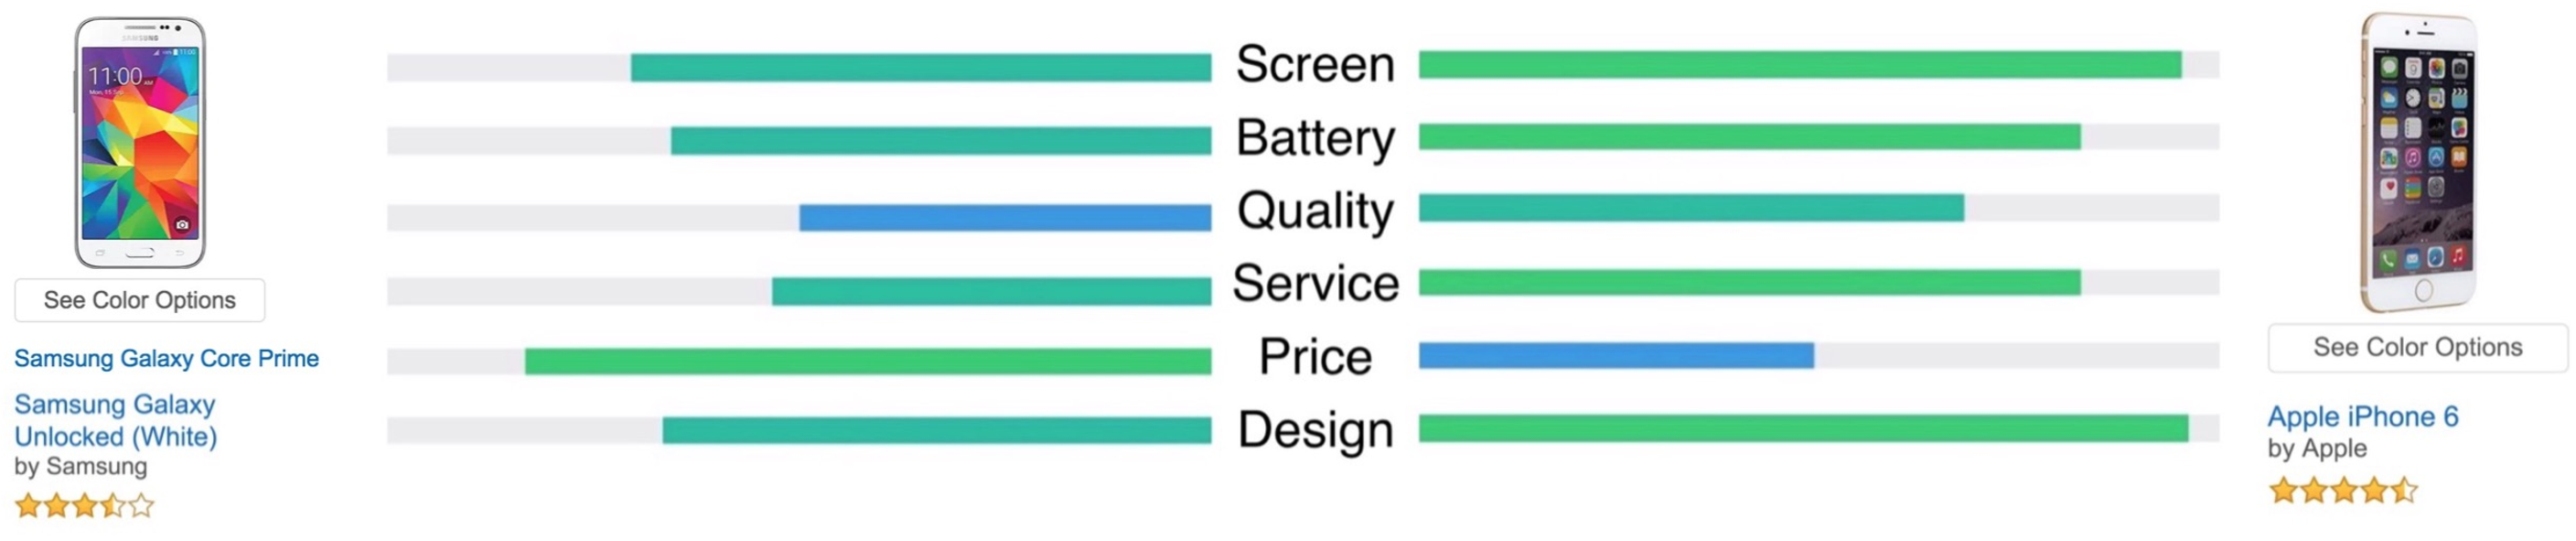
\includegraphics[width=1.0\columnwidth]{figures/comparison}
%\caption{Comparing two mobile phones.}
%\label{fig:experiments:comparison}
%\end{figure}

%\KZ{Where should the following para go? Doesn't seem very relevant to
%experiment 3. Is it a summary of the whole section? Then shouldnt start
%with Another...}
%One of the advantages of using our method for review summarization
%is that the chosen aspects 
%reflect what the consumers care most about each product type. 
%The fundamental reason behind this is that our model can truly leverage 
%the large amount of data compared to traditional methods. 
%In \figref{fig:phrases}, we can see phrases such as ``beautiful screen'' 
%and ``good camera'', but we also see ``high resolution'', which 
%is confusing because we cannot know if it means the screen or the camera, 
%and either way there is overlap in meaning. In our method, the topics of 
%the sentence is implicitly embedded in the sentence vector in the first 
%clustering process, so we can leverage not only the opinion phrases 
%but other surrounding words to decide whether ``high resolution'' 
%refers to the screen or the camera. For example, if the review 
%sentence is ``it has high resolution and the texts look so crisp'', 
%we would know it's about the screen. This allows our summarization to 
%leverage a lot more data than these traditional methods. 
